\documentclass[12pt,oneside]{book}
\usepackage{polski}
\usepackage[utf8]{inputenc}
\usepackage{fourier}
\usepackage[a4paper]{geometry}
\usepackage{geometry} % - pozwala na ustawienie parametrów strony poprzez
\geometry{verbose,a4paper,tmargin=2.5cm,bmargin=2.9cm,lmargin=5.2cm,rmargin=-.7cm}

\usepackage{fancyhdr}
\pagestyle{fancy}
\fancyhf{}

\fancypagestyle{mainmatter}{
%\rhead{Program konferencji}
\lhead{IV Ogólnopolska Konferencja Klimatologiczna}
\rfoot{\thepage}
}

\usepackage{subfiles}
\usepackage{hyperref}
\usepackage{titlesec}
\usepackage{fixltx2e}
\usepackage{longtable} 
\usepackage{pdflscape} 
\usepackage{afterpage}

\usepackage{imakeidx}
\makeindex[name=a,title=Authors,intoc=true]

\usepackage[utf8]{inputenc}
\usepackage[T1]{fontenc}
\usepackage{eurosym}
\usepackage{amsfonts, amsmath, hanging, hyperref, parskip, times}
\usepackage[numbers]{natbib}
\usepackage[pdftex]{graphicx}
\usepackage{graphicx} 
\hypersetup{
	colorlinks,
	linkcolor=black,
	urlcolor=black,
	citecolor=black
}

\usepackage{pdfpages}

%\let\section=\subsubsection
\newcommand{\pkg}[1]{{\normalfont\fontseries{b}\selectfont #1}}
\let\proglang=\textit
\let\code=\texttt
\newcommand{\atitle}[1]{\begin{center}{\bf \LARGE #1}\end{center}}
\newcommand{\affiliations}{\footnotesize\centering}

\providecommand{\tightlist}{%
	\setlength{\itemsep}{0pt}\setlength{\parskip}{0pt}}

\setlength{\topmargin}{-15mm}
\setlength{\oddsidemargin}{5mm}
\setlength{\textwidth}{165mm}
\setlength{\textheight}{250mm}

\titleformat{\chapter}[display]
{\normalfont\bfseries}{}{0pt}{\Large}

\titleformat{\section}[block]
{\Large\bfseries}{}{0pt}{\titlerule\\}[\vspace{2pt}\titlerule]

%\titleformat{\section}[block]
%{\Large\bfseries\filcenter}{}{1em}{}

\setcounter{secnumdepth}{0}
\setcounter{tocdepth}{3}

\title{IV Ogólnopolska Konferencja Klimatologiczna \\ \emph{"Aktualne problemy badawcze w meteorologii i klimatologii"}}
\vspace{12cm}
\date{Poznań, 23 marca 2018 r.}
\author{Uniwersytet im. Adama Mickiewicza w Poznaniu\\Wydział Nauk Geograficznych i Geologicznych}

\usepackage{graphicx}
\begin{document}

% 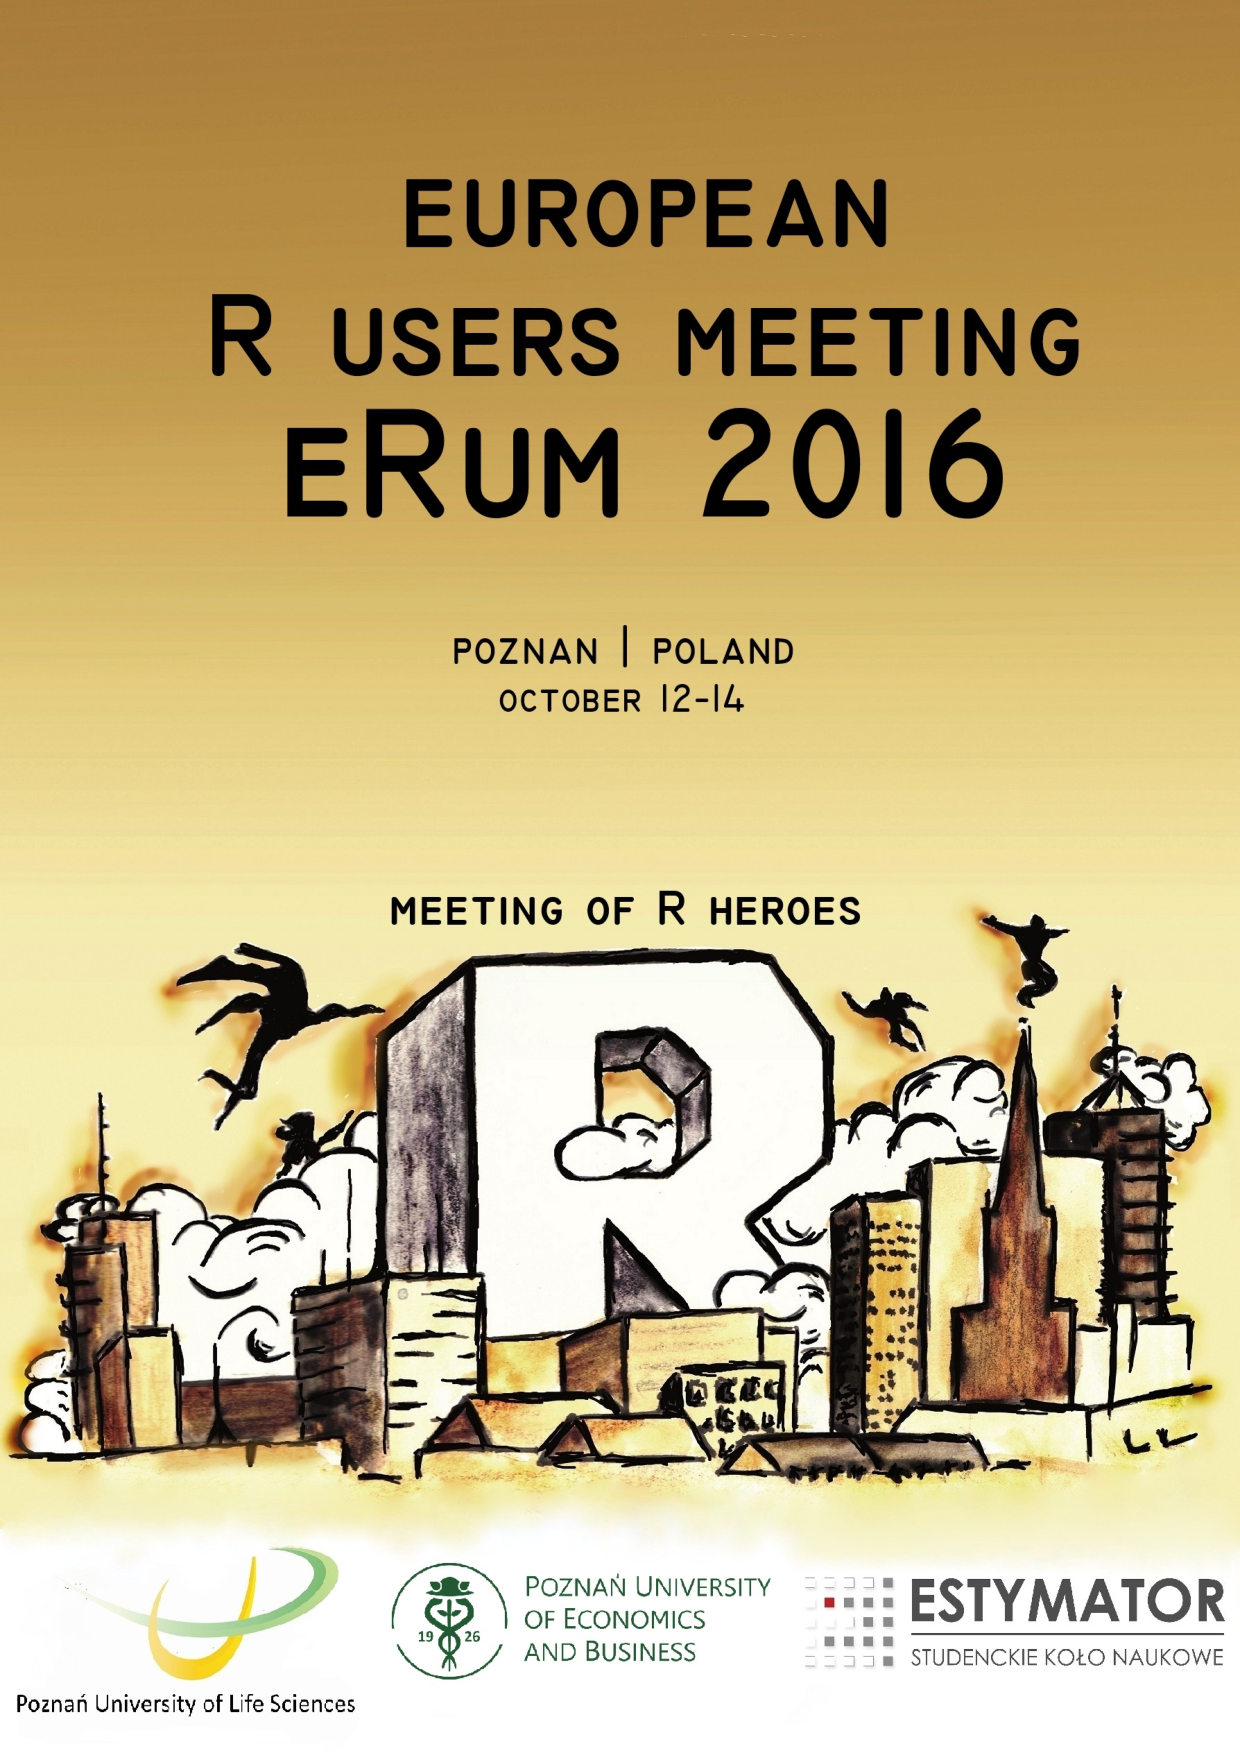
\includepdf{figs/front_cover.pdf}
% \cleardoublepage

\frontmatter
\maketitle

\chapter*{KOMITET NAUKOWY}
\vspace{-0.5cm}
prof. UAM dr hab. Leszek Kolendowicz, \textit{Uniwersytet im. Adama Mickiewicza}

prof. dr hab. Ewa Bednorz, \textit{Uniwersytet im. Adama Mickiewicza}

prof. dr hab. Krzysztof Fortuniak,  \textit{Uniwersytet Łódzki}

prof. dr hab. Joanna Wibig, \textit{Uniwersytet Łódzki}

prof. UWr. dr hab. Maciej Kryza, \textit{Uniwersytet Wrocławski}

prof. dr hab. Krzysztof Migała,  \textit{Uniwersytet Wrocławski}

prof. dr hab. Zbigniew Ustrnul,  \textit{Uniwersytet Jagielloński}

prof. dr hab. Ewa Łupikasza,  \textit{Uniwersytet Śląski}

prof. UAM dr hab. Dariusz Wrzesiński, \textit{Uniwersytet im. Adama Mickiewicza}


\vspace{2cm}
\Large{\textbf{KOMITET ORGANIZACYJNY}}
\vspace{0.5cm}

\normalsize 

mgr Sebastian Kendzierski

prof. UAM dr hab. Leszek Kolendowicz

prof dr hab. Ewa Bednorz

dr Bartosz Czernecki

dr Marek Półrolniczak

dr Katarzyna Szyga-Pluta

dr Mateusz Taszarek

dr Arkadiusz Tomczyk

mgr Hanna Forycka -- Ławniczak


%\begin{landscape}
\chapter{Szczegółowy program konferencji }

\Large{8:00 – 9:00 rejestracja uczestników\\
9:00 – 10:30 otwarcie konferencji oraz I sesja referatowa\\
10:30 – 11:00 przerwa kawowa\\
11:00 – 13:30 II  sesja referatowa \\
13:30 – 14:15 obiad\\
14:15 – 16:45 III sesja referatowa\\
16:45 – 17:00 przerwa kawowa\\
17:00 – 18:30 IV sesja referatowa\\
18:30 – 19:00 podsumowanie i zakończenie konferencji}

%% latex table generated in R 3.3.1 by xtable 1.8-2 package
% Mon Oct  3 09:55:07 2016
\begingroup\fontsize{9pt}{10pt}\selectfont
\begin{longtable}{|p{2.6cm}|p{1.8cm}|p{1.9cm}|p{2.2cm}|p{9cm}|p{2.5cm}|}
  \hline
Session & Type & Name & Surname & Title & Chairman \\ 
  \hline
  \hline
Business 1 & Regular talk & Michal & Zylinski & Turning R into production – make your models reality & Adolfo Alvarez \\ 
  Business 1 & Regular talk & Łukasz & Grala & RevoScaleR - performance and scalability R &  \\ 
  Business 1 & Regular talk & Wit & Jakuczun & Bringing R to Enterprise &  \\ 
  Business 1 & Regular talk & Erik & Barzagar-Nazari & Data science outside the box: Developing a generic scoring algorithm for customer acquisition &  \\ 
  Business 1 & Regular talk & Andreas & Wygrabek & Embedding R in business processes &  \\ 
  Business 2 & Regular talk & David & Kun & Enterprise R Platform – the what, the why and the how & Łukasz Wawrowski \\ 
  Business 2 & Regular talk & Oliver & Bracht & R in the Mittelstand: Bringing Data Science to small and mid-size companies &  \\ 
  Business 2 & Regular talk & Paweł & Ładyżyński & R tools and tricks for marketing inference in a big internet company &  \\ 
  Business 2 & Regular talk & Michał & Bryś & Using Google Analytics with R &  \\ 
  Business 2 & Regular talk & Piotr & Wójcik & Using R for backtesting algorithmic trading strategies on high-frequency data &  \\ 
  \hline
  Data Workflow 1 & Regular talk & Olgun & Aydin & Dynamic Inflation Rate Calculation of Fast-Moving Consumer Goods: Shiny-SparkR App & Marcin Kosiński \\ 
  Data Workflow 1 & Regular talk & Michał & Maj & Introduction to RDruid &  \\ 
  Data Workflow 1 & Regular talk & Anna & Wróblewska & Search phrases in e-commerce platform allegro.pl - big data analysis using SparkR &  \\ 
  Data Workflow 1 & Regular talk & Natalia & Potocka & The full process of creating an R application in recommendation systems: from Dockerfile to Zabbix monitoring &  \\ 
  Data Workflow 2 & Regular talk & Paweł & Cejrowski & Power of Java's RSession and rKafka in the data science team collaboration & Marcin Dyderski \\ 
  Data Workflow 2 & Regular talk & Ming & Shan & R Shiny for Real-time Analytics and Insight Delivery – A Solution for Complex Data in Agriculture &  \\ 
  Data Workflow 2 & Regular talk & Adam & Ryczkowski & Seamless external R server integration with Excel with step-by-step debugging of the R code &  \\ 
  Data Workflow 2 & Regular talk & Filip & Stachura & Workflow around modelling in Data Science / R &  \\ 
  \hline
  Methodology 1 & Regular talk & Maren & Eckhoff & Predicting machine failures & Marcin Szymkowiak \\ 
  Methodology 1 & Regular talk & Mateusz & Filarowski & Ensemble learning - idea and applications &  \\ 
  Methodology 1 & Regular talk & Tomasz & Smolarczyk & Ensemble learning - implementation with mlr &  \\ 
  Methodology 2 & Regular talk & Emilio L. & Cano & Unattended SVM parameters fitting for monitoring nonlinear profiles & Maciej Beręsewicz \\ 
  Methodology 2 & Regular talk & Philipp & Thomann & SimonsSVM: A Fast and Scalable Support Vector Machine Implementation for R &  \\ 
  Methodology 2 & Regular talk & Tomasz & Górecki & Multivariate analysis of variance for functional data using R &  \\ 
  Methodology 2 & Regular talk & Christoph & Hoffmann & Text Mining in R &  \\ 
  Methodology 3 & Regular talk & Adolfo & Alvarez & Classic and network based cluster analysis: together we're better &  \\ 
  Methodology 3 & Regular talk & Maciej & Beręsewicz & M-quantile regression in R &  \\ 
  Methodology 3 & Regular talk & Marcin & Dyderski & Is forest a pharmacy? - problems with data analyses &  \\ 
  Methodology 3 & Regular talk & Gero & Szepannek & k Prototypes Clustering of Mixed Type Data &  \\ 
  \hline
  Packages 1 & Regular talk & Robin & Hyndman & Reconciling forecasts: the hts package & Tomasz Górecki \\ 
  Packages 1 & Regular talk & Robin & Lovelace & stplanr: an R package for transport planning &  \\ 
  Packages 1 & Regular talk & Paul-Christian & Buerkner & brms: An R Package for Bayesian Multilevel Models using Stan &  \\ 
  Packages 1 & Regular talk & Sebastian & Warnholz & Modules in R &  \\ 
  Packages 1 & Regular talk & Massimiliano & Pastore & influence.SEM 2.0: An R Package for Sensitivity Analysis in Structural Equation Models &  \\ 
  Packages 2 & Regular talk & Rebecca & Killick & EnvCpt: An R package for changepoint identification in Environmental data & Marek Gągolewski \\ 
  Packages 2 & Regular talk & Marcin & Kosiński & archivist 2.0: News from Managing Data Analysis Results Toolkit &  \\ 
  Packages 2 & Regular talk & Daniel & Guhl & Discrete Choice Models in R &  \\ 
  Packages 2 & Regular talk & Kamil & Wais & LimeRick: Bridge between LimeSurvey and R &  \\ 
  \hline
  BioR & Regular talk & Paweł & Łabaj & Are we ready for Personalized Medicine? & Przemysław Biecek \\ 
  BioR & Regular talk & Michał & Burdukiewicz & N-gram analysis of biological sequences in R &  \\ 
  BioR & Regular talk & Stefan & Rödiger & R as an Environment for the Reproducible Analysis of DNA Amplification Experiments &  \\ 
  BioR & Regular talk & Marek & Wiewiórka & Big data genomics data warehouses analyses with R &  \\ 
  BioR & Regular talk & Michal & Okoniewski & Using SparkR with distributed database in Parquet - a genomic example &  \\ 
  \hline
  Education Learning & Regular talk & Filip & Schouwenaars & Revolutionize how you teach and blog: add interactivity & Alicja Szabelska-Beręsewicz \\ 
  Education Learning & Regular talk & Martin & Schneider & Aargh I have to teach R (Experiences in the teaching of R) &  \\ 
  Education Learning & Regular talk & Päivi & Julin & Using R for artistic purposes &  \\ 
  Education Learning & Regular talk & Kamil & Krawczyk & Polish Diet Commissions - Text Analysis &  \\ 
  \hline
  Lightning talks & Lightning talk & Agnieszka & Borsuk & R as a tool for graphical diagnostics in population pharmacokinetic modeling & Joanna Zyprych-Walczak \\ 
  Lightning talks & Lightning talk & Bartosz & Czernecki & Machine learning modeling of phenological phases in Poland &  \\ 
  Lightning talks & Lightning talk & Paweł & Kleka & Latent Class Analysis in Psychology &  \\ 
  Lightning talks & Lightning talk & Bogumil & Konopka & Exploratory data analysis of a clinical study group - revealing patient subgroups. &  \\ 
  Lightning talks & Lightning talk & Alexander & Kruse & Multidimensional Clustering of Web Analytics Data &  \\ 
  Lightning talks & Lightning talk & Giovanni & Lotti & R shiny server as core of multiple technologies into Travel Industry. &  \\ 
  Lightning talks & Lightning talk & George & Moroz & Turning Text Mining into Language Mining: Corpus Linguistics in R &  \\ 
  Lightning talks & Lightning talk & Paweł & Piątkowski & Structural bioinformatician's notebooks with pdbeeR and knitr &  \\ 
  Lightning talks & Lightning talk & Paul & Roback & Using R to incorporate data science into the undergraduate statistics curriculum &  \\ 
  Lightning talks & Lightning talks & Luigi & Lombardi & Analysing the statistical effects of manipulated data &  \\ 
  Lightning talks & Lightning talks & Jaroem & Ooms & Cryptography in R &  \\ 
  Lightning talks & Lightning talk & Piotr & Sobczyk & Visualizing changes in demographics with R &  \\ 
  Lightning talks & Lightning talk & Zofia & Tylutki & R for pharmacokineticists - smulation of steady-state concentrations of amiodarone in heart compartmental model as an example. &  \\ 
  \hline
  Poster session & Poster & Damian & Chmura & What are sampling errors in the vegetation studies using visual estimation of presence and cover of plants? R can help &  \\ 
  Poster session & Poster & Carolina & Correia & RNA-seq transcriptional profiling of PPD-b-stimulated peripheral blood from cattle infected with Mycobacterium bovis &  \\ 
  Poster session & Poster & Emilia & Daghir-Wojtkowiak & Pharmacokinetics-driven modeling of metabolomics data &  \\ 
  Poster session & Poster & Anna & Dmowska & R as a tool for geospatial modeling in large dataset - example of dasymetric modeling at a continental scale (United States) &  \\ 
  Poster session & Poster & Dimitri & Fichou & Application of Artificial Neural Network to Planar Chromatography Data &  \\ 
  Poster session & Poster & Jagoda & Jabłońska & cgmisc: enhanced genome-wide association analyses and visualization &  \\ 
  Poster session & Poster & Marta & Karas & Penalized regression inference regarding variable selection in regular and high dimensions: comparison of selected methods implemented in R &  \\ 
  Poster session & Poster & Wojciech & Kędziora & Wrestling with big data in forestry: use of R in Scots pine site index analysis. &  \\ 
  Poster session & Poster & Tomasz & Owczarek & An R implementation of Kauffman's NK model &  \\ 
  Poster session & Poster & Anna & Rybińska & R as an effective data mining tool in chemistry &  \\ 
  Poster session & Poster & Fabián & Santos & Applying genetic algorithms to calibrate a processing chain for a Landsat-based time series analysis of disturbance - regrowth dynamics in tropical forests &  \\ 
  Poster session & Poster & Sylwia & Wierzcholska & Modelling the distrubution of the bryophytes in different spatial scales &  \\ 
  Poster session & Poster & Daniel & Rabczenko & Mortality mapping using R &  \\ 
  \hline
\hline
\end{longtable}
\endgroup

%\end{landscape}
%\chapter{Przedmowa}
%\Large
\raggedright Szanowni Uczestnicy,

\vspace{1cm}

W imieniu Komitetu Naukowego oraz Organizacyjnego mamy zaszczyt zaprosić Państwa na IV
Ogólnopolską  Konferencję  Klimatologiczną pt. \emph{ "Aktualne    problemy    badawcze w meteorologii i klimatologii"}.

Celem  konferencji  jest  prezentacja  wyników  badań  młodych  naukowców  z  zakresu meteorologii  i  klimatologii. Konferencja  skierowana jest  dla  doktorantów  oraz  studentów  studiów magisterskich (II stopnia) z zakresu meteorologii i klimatologii. 

\vspace{1cm}

Życzymy owocnych obrad!

\vspace{4.5cm}

\large
\begin{flushright}
mgr Sebastian Kendzierski \\
Przewodniczący Komitetu Organizacyjnego \\ 
\end{flushright}


\large{
\tableofcontents
}
\mainmatter

\pagestyle{mainmatter}% mainmatter page style


\chapter{Abstrakty}
\large
\vspace{-0.5cm}
\subfile{abstrakty/Bielecki.tex} \label{bielecki}
\newpage
\subfile{abstrakty/Bilinska.tex} \label{bilinska}
\newpage
\subfile{abstrakty/Dziembor.tex} \label{dziembor}
\newpage
\subfile{abstrakty/Franczyk.tex} \label{franczyk}
\newpage
\subfile{abstrakty/Guzik.tex} \label{guzik}
\newpage
\subfile{abstrakty/Kolendowicz.tex} \label{kolendowicz}
\newpage
\subfile{abstrakty/Plewa.tex} \label{plewa}
\newpage 	
\subfile{abstrakty/Poreba.tex} \label{poreba}
\newpage 	
\subfile {abstrakty/Skomorowski.tex} \label{skomorowski}
\newpage
\subfile{abstrakty/Wieczorek.tex} \label{wieczorek}
\newpage
\subfile{abstrakty/Sekowski.tex} \label{sekowski}
\newpage
\subfile{abstrakty/Swider.tex} \label{swider}
\newpage
\subfile{abstrakty/Pawliczek.tex} \label{pawliczek}
\newpage
\subfile{abstrakty/Cybulski.tex} \label{cybulski}
\newpage
\subfile{abstrakty/Piasecki.tex} \label{piasecki}
\newpage
%\subfile{abstrakty/Pilorz.tex} \label{pilorz}
%\newpage
\subfile{abstrakty/Sypniewski.tex} \label{sypniewski}



\chapter{Uczestnicy konferencji}

Kolejność uczestników w porządku alfabetycznym:


\normalsize
\begin{tabular}{||c|l|l|l||}
\hline
\hline
\textbf{lp.} & \textbf{imię i nazwisko} & \textbf{afiliacja} & \textbf{forma}\\
 &  &  & \textbf{uczestnictwa}\\
\hline
\hline
\hline
	 & Ewa Bednorz & Uniwersytet im. A. Mickiewicza & referat \\\hline
	 & Rafał Bielecki & Uniwersytet Pedagogiczny & referat (str. \pageref{bielecki})\\
	 &  & w Krakowie & -- \\\hline
	 & Daria Bilińska & Uniwersytet Wrocławski & referat (str. \pageref{bilinska}) \\\hline
	 & Paulina Bryś & Uniwersytet Jagielloński & -- \\\hline
	 & Bartłomiej Cybulski & Politechnika Łódzka & referat (str. \pageref{cybulski}) \\\hline
	 & Kaja Czarnecka & Uniwersytet Warszawski & -- \\\hline
	 & Bartosz Czernecki & Uniwersytet im. A. Mickiewicza & referat (str. \pageref{kolendowicz}) \\\hline
 	 & Katarzyna Dziembor & Uniwersytet Gdański, & referat (str. \pageref{dziembor})\\
		 &  & Polska Akademia Nauk &  \\\hline
 	 & Wioleta Franczyk & Uniwersytet im. A. Mickiewicza & referat  (str. \pageref{franczyk})\\\hline
 	 & Izabela Guzik & Uniwersytet Jagielloński & poster/referat (str. \pageref{guzik})\\\hline	
 	 & Agnieszka Halaś & Uniwersytet Warszawski & -- \\\hline	
 	 & Leszek Kolendowicz & Uniwersytet im. A. Mickiewicza & referat (str. \pageref{kolendowicz}) \\\hline
 	 & Jakub Majchrzak & Uniwersytet Warszawski & -- \\\hline	
	 & Paulina Okońska & Uniwersytet Śląski & -- \\\hline
 	 & Piotr Pawliczek & Uniwersytet Wrocławski & referat (str. \pageref{pawliczek})\\\hline
 	 & Iwona Pawlik & Uniwersytet Śląski & -- \\\hline
 	 & Krzysztof Piasecki & Uniwersytet Warszawski, & referat (str. \pageref{piasecki})\\
		 &  & Skywarn Polska &  \\\hline
	 & Wojciech Pilorz & Uniwersytet Śląski, & referat (str. \pageref{piasecki})\\
	 &  & Skywarn Polska &  \\\hline
  	 & Katarzyna Plewa & Uniwersytet im. A. Mickiewicza & referat  (str. \pageref{plewa})\\\hline
	 & Szymon Poręba & Uniwersytet Jagielloński & referat (str. \pageref{poreba}) \\\hline
	 & Marek Półrolniczak & Uniwersytet im. A. Mickiewicza & referat (str. \pageref{kolendowicz}) \\\hline
 	 & Aleksandra Renc & Uniwersytet Śląski & -- \\\hline
	 & Oskar Sękowski & Uniwersytet Jagielloński & referat (str. \pageref{sekowski}) \\\hline
	 & Adam Skomorowski & Uniwersytet Łódzki & referat (str. \pageref{skomorowski}) \\\hline	
	 & Marta Sobkowiak & Politechnika Śląska & -- \\\hline
	 & Jakub Sypniewski & Uniwersytet im. A. Mickiewicza & referat (str. \pageref{sypniewski}) \\\hline
	 & Wojciech Szydłowski & Uniwersytet Jagielloński & -- \\\hline
	 & Kryspin Świder & Uniwersytet Przyrodniczy we Wrocławiu & referat (str. \pageref{swider}) \\\hline
	 & Mateusz Taszarek & Uniwersytet im. A. Mickiewicza & referat \\\hline
 	 & Krzysztof Wardzyński & Uniwersytet Warszawski & -- \\\hline
   & Luiza Wieczorek & Uniwersytet Łódzki & referat (str. \pageref{wieczorek}) \\\hline
   & Dariusz Zajączkowski & Uniwersytet Śląski & -- \\\hline
	
\hline
\hline
\end{tabular}

\printindex[a]
%\Large
\raggedright Indeks autorów i uczestników konferencji,

TODO

\vspace{1.5cm}




\backmatter



%
\includepdf{figs/back_cover.pdf}

\end{document}
